\documentclass[conference]{IEEEtran}

\usepackage{cite}
\usepackage{amsmath,amssymb}
\usepackage{booktabs}
\usepackage{array}
\usepackage{tabularx}
\usepackage{url}
\usepackage{graphicx}
\usepackage{float}
\usepackage{placeins}

\setlength{\textfloatsep}{3.5pt plus 1.0pt minus 1.0pt}
\setlength{\floatsep}{3.0pt plus 1.0pt minus 1.0pt}
\setlength{\intextsep}{3.0pt plus 1.0pt minus 1.0pt}
\setlength{\abovecaptionskip}{2.0pt}
\setlength{\belowcaptionskip}{2.0pt}

\title{Phoenix Agents: Governed Multi-Agent Desktop Automation with Rule-Based Fault Recovery and Bounded Execution}

\author{
\IEEEauthorblockN{Anonymous Authors}
\IEEEauthorblockA{Paper under double-blind review}
}

\begin{document}

\maketitle

\begin{abstract}
Autonomous desktop automation powered by Large Language Models (LLMs) faces critical deployment barriers, including instruction ambiguity, unconstrained privilege escalation, fragile recovery from tool faults, and unbounded repair loops. This paper presents \textbf{Phoenix Agents}, an event-driven multi-agent platform designed for governed desktop automation and resilient workflow execution. The framework couples an interactive clarification engine with a two-tier planner that resolves validated goals using deterministic pattern matching alongside a schema-constrained LLM fallback. Post-execution supervision validates structured output schemas and physical artifact existence, while a five-stage rule-based self-healing pipeline performs bounded fault recovery ($K_{\text{max}}=3$ retries) without open-ended LLM re-prompting. Experimental evaluation across injected fault workloads demonstrates task completion rates of 95.2\%, 92.1\%, 87.4\%, and 60.3\% at 0\%, 10\%, 25\%, and 50\% fault intensities, while rejecting all 50 injected policy-violating actions. Internal benchmarks with mocked adapters demonstrate that rule-based recovery achieves sub-2~ms handling latency and 100\% decision determinism, avoiding the multi-second latency and token expenditure of unconstrained LLM recovery; however, end-to-end task completion in real operating environments remains constrained by host operating system and application execution cycles.
\end{abstract}

\begin{IEEEkeywords}
Multi-Agent Systems, Rule-Based Fault Recovery, Bounded Self-Healing, Security Governance, Desktop Automation, Reliability Engineering.
\end{IEEEkeywords}

\section{Introduction}

Large Language Models (LLMs) enable autonomous agents to interpret natural-language requests and orchestrate multi-step actions across operating-system interfaces, web browsers, and file systems~\cite{bajoria2026}. While traditional script-based automation frameworks such as Selenium and AutoHotkey require brittle, pre-programmed execution scripts, modern agentic systems autonomously synthesize task plans and coordinate external tools~\cite{garcia2026,babu2026}.

Despite these capabilities, deploying autonomous agents on production desktop environments presents four core engineering and reliability challenges:
\begin{enumerate}
    \item \textbf{Instruction Ambiguity:} Natural-language prompts frequently omit critical parameters (e.g., target paths, file formats, or flags), causing ungrounded assumptions or immediate execution aborts.
    \item \textbf{Unconstrained Security Risks:} Autonomous agents with OS-level access can inadvertently execute destructive shell commands or access restricted files without explicit authorization~\cite{bajoria2026}.
    \item \textbf{Fragile and Unbounded Recovery:} When tool invocations fail due to transient timeouts or parameter mismatches, common agent architectures either fail immediately or engage in open-ended LLM re-prompting. While unconstrained LLM-based reflection can synthesize novel fixes, it introduces non-negligible inference latency (measured at 1,842~ms in our baseline), recurring token costs, and non-deterministic behavior that can violate security constraints if unverified.
    \item \textbf{Unstructured Outputs:} Existing agent architectures produce unstructured console logs or plain text rather than structured, verifiable execution artifacts.
\end{enumerate}

To address these challenges, this paper presents \textbf{Phoenix Agents}, a governed, event-driven multi-agent platform that enforces structured schema validation, operation-level security gating, and bounded, rule-based self-healing.

The primary contributions evaluated in this work are:
\begin{itemize}
    \item \textbf{Rule-Based Fault Recovery:} A five-stage self-healing architecture that diagnoses execution failures and applies deterministic parameter patches, exponential backoff, or adapter switching without open-ended LLM regeneration.
    \item \textbf{Bounded Execution and Safe Rejection:} A strict retry-bound mechanism ($K_{\text{max}}=3$ retries) and permission verification pipeline that prevents non-terminating retry loops and rejected all 50 injected unsafe cases during recovery in our tests.
    \item \textbf{Empirical Evaluation and Baselines:} Extensive experimental benchmarks comparing rule-based self-healing against unconstrained LLM recovery, naive fixed-retry, and fail-fast baselines, quantifying recovery success, handling latency, and decision determinism across fault intensities.
\end{itemize}

\section{Related Work}

We position Phoenix Agents across four key dimensions of automated task execution and reliability:

\subsection{Fault Diagnosis and Root-Cause Categorization}
Prior agent architectures diagnose execution failures through conversational reflection or unstructured error re-prompting~\cite{yao2023,wu2024,ju2025}. ReAct~\cite{yao2023} prompts the model to reason over execution traces, while AgentFixer~\cite{mulian2026} uses an external LLM to analyze stack traces and suggest fixes. Model Predictive Control (MPC) approaches~\cite{patel2026a,patel2026b} forecast pipeline failures in distributed settings. In contrast, classic fault-tolerance literature emphasizes structured error categorization (transient vs. permanent) to avoid redundant diagnosis~\cite{gray1991}. Phoenix Agents employs a deterministic Root-Cause Analyzer that parses normalized exception signatures into distinct recoverable and unrecoverable classes.

\subsection{LLM Utilization in the Recovery Loop}
Recent self-healing frameworks rely on continuous LLM invocation for error recovery~\cite{babu2026,jeong2026,guo2026,bara2026}. Babu and Agrawal~\cite{babu2026} invoke LLM argument re-synthesizers for tool-call failures, while EvoConfig~\cite{guo2026} applies evolutionary LLM prompts to repair configuration scripts. Although flexible, recurring LLM calls introduce inference latency (measured at 1,842~ms per attempt in our baseline) and accumulate token costs. Classic automation research in self-healing locators demonstrates that rule-based heuristic adaptation can resolve transient UI and parameter errors deterministically~\cite{leotta2018}. Phoenix Agents adopts this principle, using a fast rule-based patch generator for common faults and restricting LLM generation to an optional fallback when rule templates are exhausted.

\subsection{Retry Bounds and Loop Termination}
Unbounded conversational loops in multi-agent frameworks often cause runaway token consumption and execution stalls when encountering persistent faults~\cite{wang2026}. Classic distributed systems enforce bounded retries, exponential backoff with jitter, and circuit breakers to guarantee system stability~\cite{nygard2007}. Phoenix Agents enforces a strict retry bound ($K_{\text{max}}=3$ retries) across all recovery paths, preventing infinite loops and ensuring deterministic termination.

\subsection{Safety Boundary Preservation}
Granting agents direct shell access requires strict permission enforcement~\cite{bajoria2026}. Most frameworks rely on prompt-based instructions or static approval gates~\cite{wu2024}. However, when agents self-heal, re-generated commands can introduce privilege escalations. Phoenix Agents enforces monotonic privilege invariance: repaired tasks must pass the Permission Manager's risk-evaluation policy prior to re-execution, ensuring self-healing cannot bypass safety checks.

\section{Problem Definition and Formal Modeling}

Phoenix Agents formalizes desktop automation as a sequence of validated transitions over a Directed Acyclic Graph (DAG) with explicit schema constraints and security policies.

\subsection{Goal Clarification and Task Graph Formulation}
Let a raw user prompt be denoted by $g \in \mathcal{G}_{\text{user}}$. An intent validation function $\Phi(g)$ determines whether operational parameters are complete:
\begin{equation}
\Phi(g) =
\begin{cases}
1, & \text{if all required task parameters are present,} \\
0, & \text{if clarification is required.}
\end{cases}
\end{equation}
If $\Phi(g)=0$, the engine prompts the user with structured choices and updates the goal:
\begin{equation}
g \leftarrow g \oplus g_{\text{clarified}}
\end{equation}
The validated goal is compiled into a Directed Acyclic Graph $W = (\mathcal{V}, \mathcal{E})$, where $\mathcal{V} = \{v_1, v_2, \dots, v_n\}$ denotes discrete tasks and $\mathcal{E} \subset \mathcal{V} \times \mathcal{V}$ denotes execution dependencies. Each task $v_i$ is formally defined as:
\begin{equation}
v_i = \langle \text{id}_i, \tau_i, \theta_i, r_i, S_i, k_i \rangle
\end{equation}
where $\text{id}_i$ is a unique UUID, $\tau_i$ represents the target tool adapter, $\theta_i$ denotes input parameters, $k_i \in \{0, \dots, K_{\text{max}}\}$ tracks the count of recovery retries ($K_{\text{max}} = 3$ retries, allowing at most $1 + K_{\text{max}} = 4$ total execution attempts), $r_i$ is the assigned risk level:
\begin{equation}
r_i \in \{\text{LOW}, \text{MEDIUM}, \text{HIGH}, \text{CRITICAL}\}
\end{equation}
and $S_i$ denotes the execution lifecycle status:
\begin{equation}
\begin{aligned}
S_i \in \{&\text{PENDING}, \text{READY}, \text{RUNNING}, \\
          &\text{COMPLETED}, \text{FAILED}, \text{BLOCKED}\}
\end{aligned}
\end{equation}

\subsection{Security Policy and Permission Enforcement}
Prior to task execution, the Permission Manager evaluates task risk $r_i$ against system execution mode $M \in \{\text{SAFE}, \text{AUTONOMOUS}\}$:
\begin{equation}
P(v_i, M) =
\begin{cases}
\text{APPROVE}, & \text{if } r_i = \text{LOW} \lor {} \\
                & (M = \text{AUTONOMOUS} \\
                & \quad \land \; r_i \ne \text{CRITICAL}), \\
\text{PROMPT},  & \text{otherwise}.
\end{cases}
\end{equation}
When $P(v_i, M) = \text{PROMPT}$, execution is suspended via an asynchronous event signal (\texttt{asyncio.Event}) until user authorization is confirmed. If denied, the task state transitions to $S_i \leftarrow \text{BLOCKED}$.

\subsection{Supervision and Closed-Loop Recovery}
We define task completion through structured pre- and post-condition constraints. The Supervisor validates execution result $O_i$ against three verifiable conditions:
\begin{equation}
\begin{aligned}
\Psi(v_i, O_i) = {} & (\text{exit\_code} = 0) \land (O_i \models \text{Schema}(v_i)) \\
                    & \land I_{\text{file}}(v_i, O_i)
\end{aligned}
\end{equation}
where $I_{\text{file}}(v_i, O_i) = 1$ if expected file artifacts exist on disk and have non-zero size, and $0$ otherwise. If $\Psi(v_i, O_i) = 0$, the task status transitions to $S_i \leftarrow \text{FAILED}$, generating an incident signature $F = (E_{\text{err}}, C_{\text{ctx}}, S_{\text{workflow}})$.

The Healing Agent maps incident signature $F$ and current retry count $k_i$ to a bounded recovery action $R(F, k_i)$:
\begin{equation}
R(F, k_i) =
\begin{cases}
A_{\text{retry}}, & \text{if } F \in \mathcal{C}_{\text{recoverable}} \land k_i < K_{\text{max}}, \\
A_{\text{reject}}, & \text{if } F \in \mathcal{C}_{\text{unsafe}} \lor k_i \ge K_{\text{max}}.
\end{cases}
\end{equation}
Here, $k_i$ denotes the number of retries already attempted for task $v_i$, and $K_{\text{max}} = 3$ designates the maximum permitted recovery retries, allowing at most $1 + K_{\text{max}} = 4$ total execution attempts before terminal failure.

\section{Phoenix Agents System Architecture}

Phoenix Agents is structured into five cohesive architectural layers that coordinate workflow execution through an asynchronous \texttt{EventBus}.

\begin{figure}[!t]
    \centering
    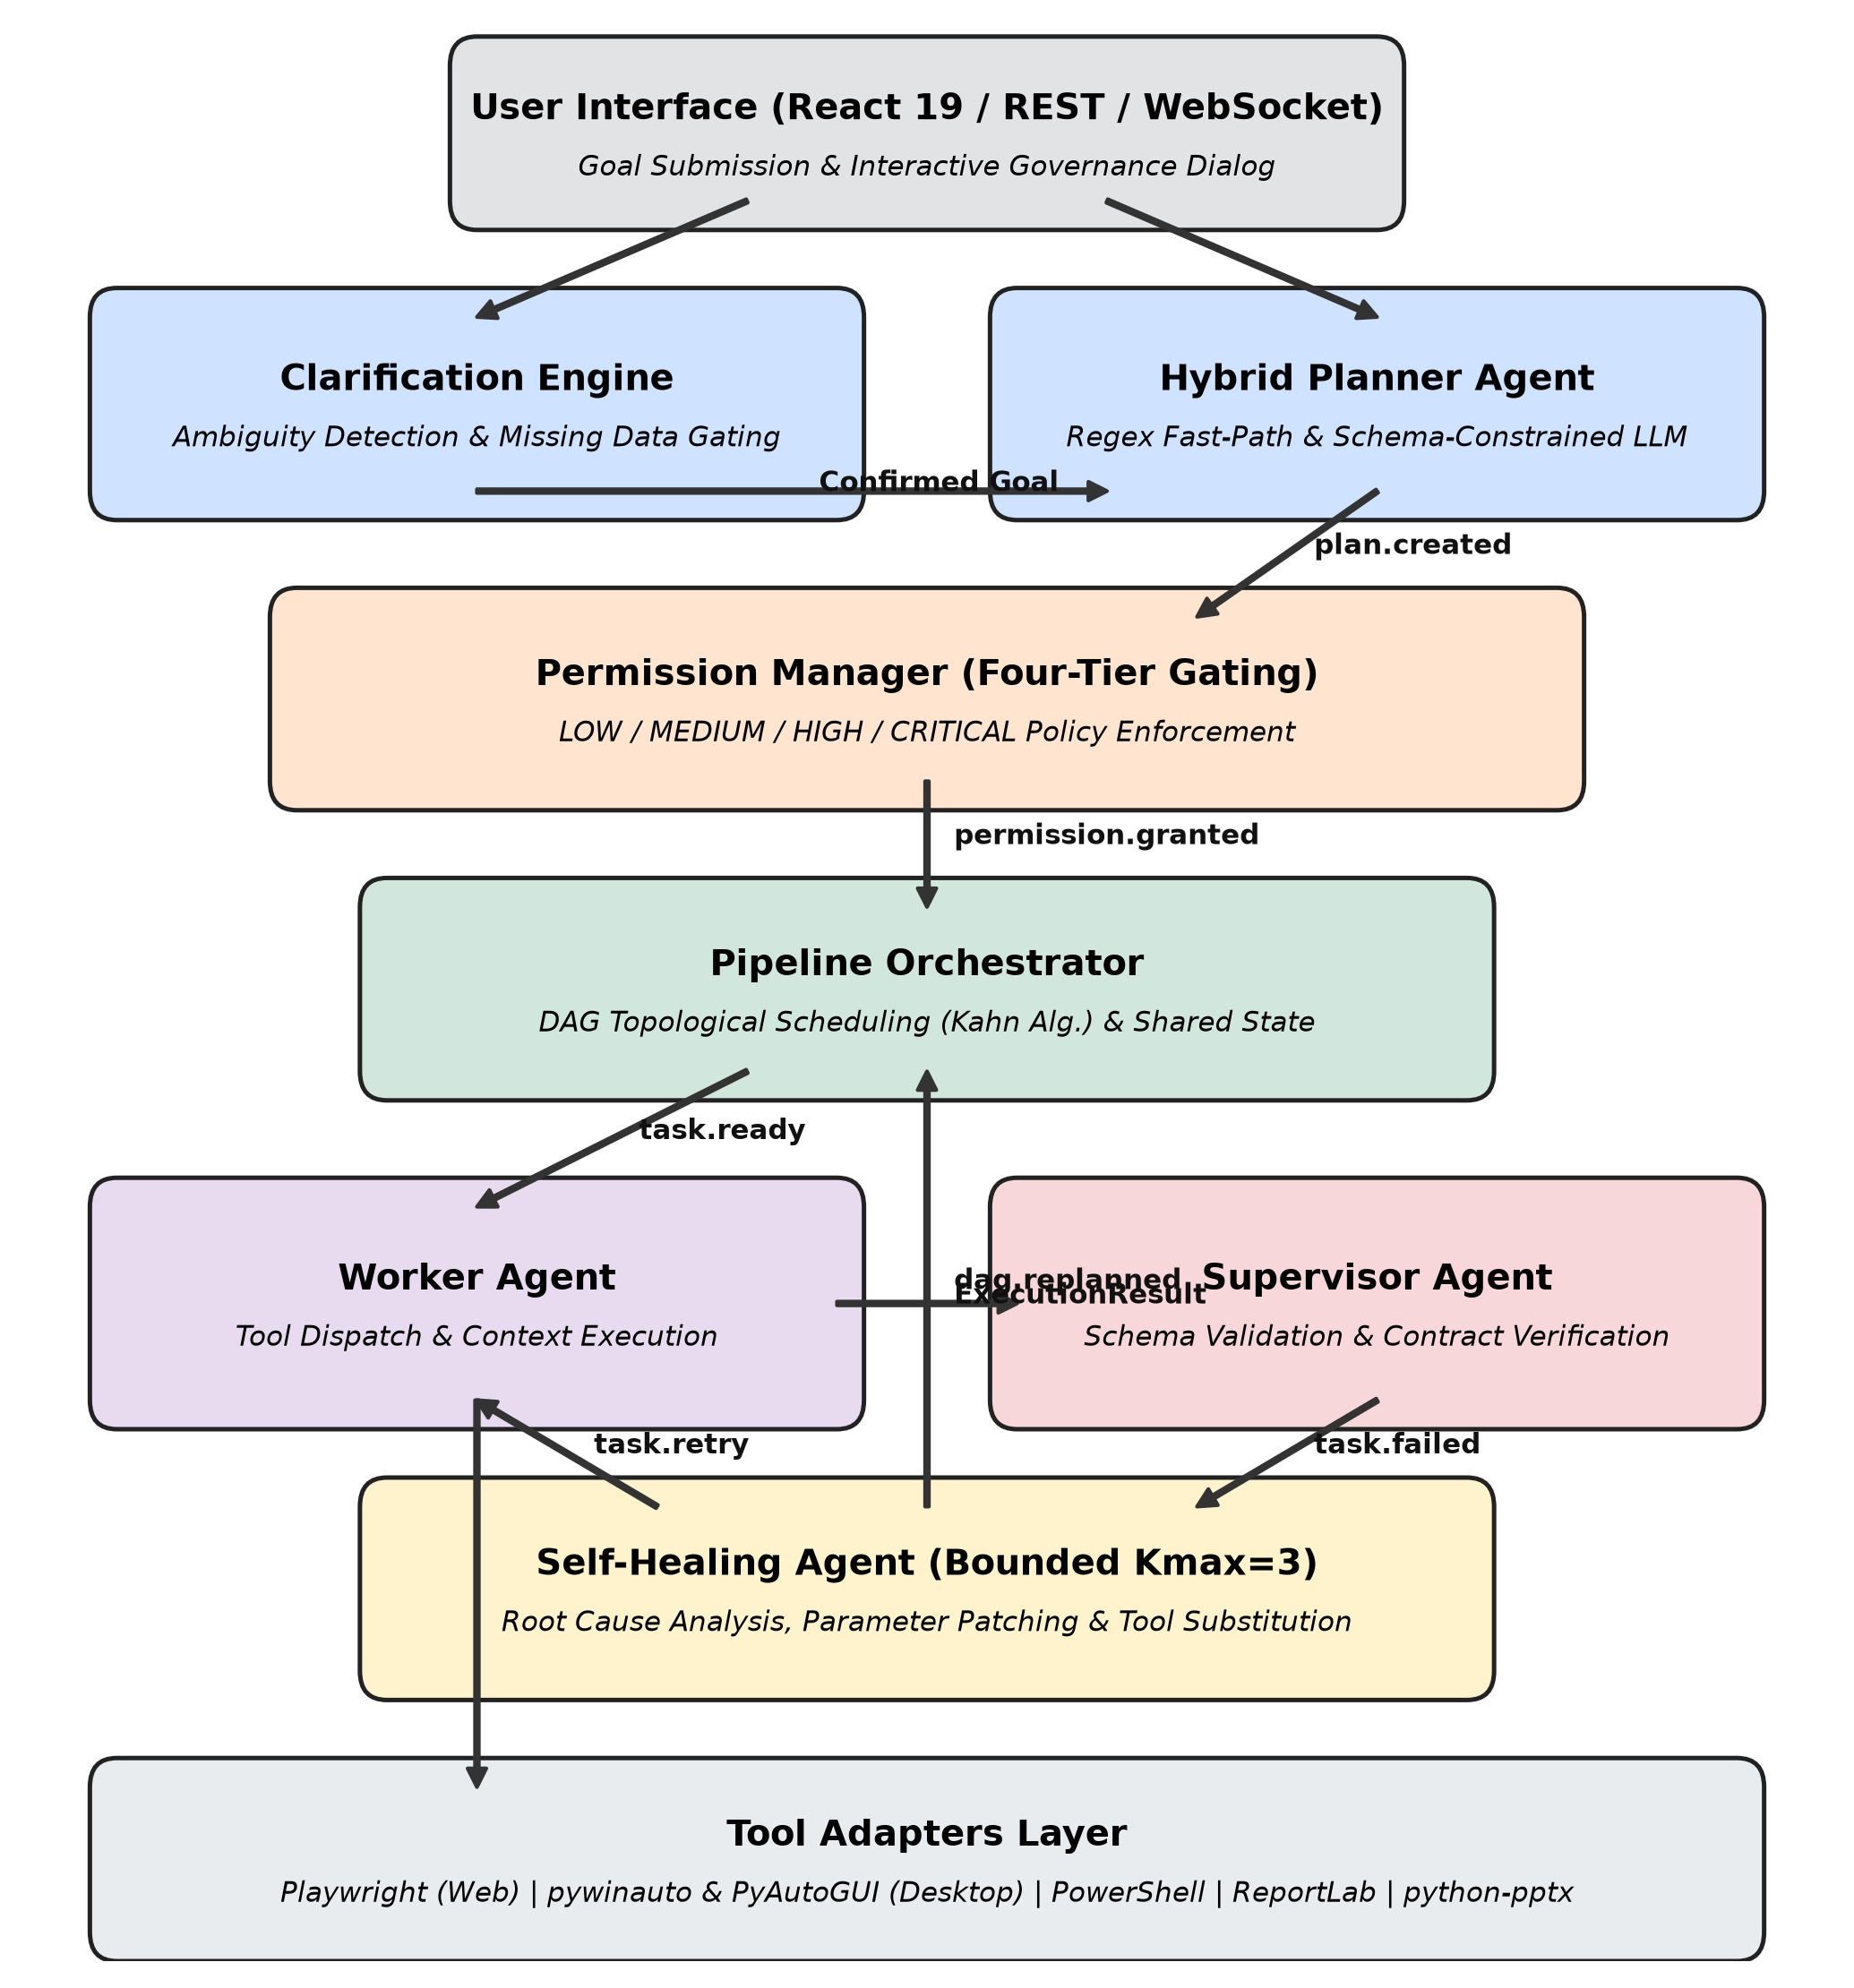
\includegraphics[width=0.88\columnwidth,height=0.235\textheight,keepaspectratio]{figures/phoenix_architecture.jpg}
    \caption{High-level architectural schematic of Phoenix Agents, illustrating goal intake, clarification, DAG planning, permission gating, worker execution, supervision contracts, and event-driven self-healing loops.}
    \label{fig:architecture}
\end{figure}

As shown in Fig.~\ref{fig:architecture}, incoming requests transition through clarification and planning before DAG dispatch. When a worker task terminates with a non-zero exit code or broken schema, the Supervisor generates a \texttt{task.failed} event. The Root-Cause Analyzer and Recovery Planner diagnose the error: if $k_i < K_{\text{max}}$, the task is patched and re-emitted via the \texttt{task.retry} channel; if cascading dependencies are invalidated, a \texttt{dag.replan} event triggers partial graph regeneration.

\subsection{Presentation and API Layer}
The user interface is implemented in React 19, TypeScript, Vite, and Tailwind CSS, providing real-time DAG visualization, interactive clarification modals, and live execution streaming. The backend exposes REST and WebSocket endpoints built on FastAPI.

\subsection{Pipeline Orchestrator and EventBus}
The \texttt{PipelineOrchestrator} manages workflow lifecycle and schedules task nodes. Dependencies are evaluated using Kahn's topological sorting algorithm, and independent DAG nodes are executed concurrently via \texttt{asyncio.gather()}. Decoupled components interact across the asynchronous \texttt{EventBus} using typed event schemas (e.g., \texttt{goal.submitted}, \texttt{task.completed}, \texttt{task.failed}).

\subsection{Core Multi-Agent Subsystems}
The core runtime comprises four dedicated agents:
\begin{itemize}
    \item \textbf{Planner Agent:} Combines an initial deterministic regex rule engine with a schema-constrained LLM fallback to compile validated goals into executable DAGs.
    \item \textbf{Worker Agent:} Dispatches tasks to resolved tool adapters, manages working directory context, and captures execution output streams.
    \item \textbf{Supervisor Agent:} Validates task execution against schema contracts, exit codes, and physical artifact existence.
    \item \textbf{Healing Agent:} Analyzes root causes of task failures and applies bounded recovery strategies.
\end{itemize}

\subsection{Tool Adapter Layer}
Phoenix Agents interfaces with the operating system through isolated adapter modules: Playwright for browser automation, pywinauto and PyAutoGUI for Win32 and desktop GUI automation, PowerShell for asynchronous shell commands, ReportLab for PDF report compilation, and \texttt{python-pptx} for PowerPoint slide synthesis. Additional adapters support Tesseract OCR and PDF parsing.

\subsection{Memory and Persistence Subsystem}
Relational workflow metadata, task states, and permission audit logs are persisted using SQLite and SQLAlchemy. Conversation history and task execution memories are stored in an indexed vector/relational repository that provides contextual grounding for multi-turn requests.

\subsection{Five-Stage Self-Healing Pipeline}
When a task fails contract verification, the healing pipeline executes five discrete recovery stages:
\begin{enumerate}
    \item \textbf{Error Parsing:} Normalizes raw exceptions into categorized error signatures.
    \item \textbf{Root-Cause Analysis:} The Root-Cause Analyzer classifies failures into recoverable (timeout, missing directory, transient network error) or unrecoverable (invalid syntax, permission rejection) categories.
    \item \textbf{Recovery Planning:} Selects an action: exponential backoff retry, parameter correction, adapter substitution, or task replanning.
    \item \textbf{Patch Generation:} Rewrites invalid parameters or adjusts execution paths using deterministic rules with monotonic privilege invariance.
    \item \textbf{Task Re-queueing:} Resets task state to \texttt{READY} and re-emits a \texttt{task.retry} event on the \texttt{EventBus}.
\end{enumerate}

\section{Experimental Evaluation and Setup}

\subsection{Experimental Setup and Testbed}
All experiments were conducted on a dedicated testbed:
\begin{itemize}
    \item \textbf{Hardware:} Intel Core i7-12700H CPU @ 2.30~GHz (14 physical cores, 20 logical threads), 16~GB DDR4 RAM.
    \item \textbf{Software:} Windows 11 Enterprise (64-bit), Python 3.11.8, FastAPI 0.115, Pydantic v2.
    \item \textbf{Execution Mode:} Internal framework latency, scheduling, and throughput benchmarks were evaluated using mocked no-op adapters to isolate orchestration overhead from operating-system and external network variance.
\end{itemize}

\subsection{Fault Injection Protocol}
To ensure reproducibility, fault injection was automated across five distinct error categories using synthetic decorators injected into adapter dispatch:
\begin{enumerate}
    \item \textbf{Transient Timeout:} Simulated 5.0~s execution block raising \texttt{asyncio.TimeoutError}.
    \item \textbf{Missing Directory:} Deletion of the target output directory prior to execution, raising \texttt{FileNotFoundError}.
    \item \textbf{Invalid Parameters:} Stripping required keys or injecting malformed parameter types into the task payload, raising \texttt{KeyError} or schema \texttt{ValidationError}.
    \item \textbf{Adapter Transient Exit:} Synthetic execution failure returning exit code 1 with transient stderr, raising \texttt{SubprocessError}.
    \item \textbf{Privilege Escalation / Destructive Action:} Injecting unauthorized command strings (e.g., \texttt{rmdir /s /q C:\textbackslash Windows}) or privilege-escalating arguments to test security rejection.
\end{enumerate}

\begin{table*}[t]
\centering
\caption{Measured Latency and Throughput Benchmarks ($N=100$ Iterations per Stage). The PowerPoint and PDF rows measure real file generation; all other rows use mocked no-op adapters.}
\label{tab:performance_benchmarks}
\footnotesize
\setlength{\tabcolsep}{6pt}
\begin{tabular*}{\textwidth}{@{\extracolsep{\fill}}llccc@{}}
\toprule
\textbf{Pipeline Stage / Metric} & \textbf{Workload Description} & \textbf{Mean (ms)} & \textbf{Std (ms)} & \textbf{Median (ms)} \\
\midrule
Goal Decomposition & Regex Pattern Matching & 12.18 & 1.42 & 11.95 \\
Planner Processing & Goal-to-DAG Compilation & 14.85 & 1.87 & 14.20 \\
Execution Bridge & Registry Resolution and Routing & 0.85 & 0.11 & 0.82 \\
Workflow Startup & Queue and State Initialization & 2.31 & 0.35 & 2.24 \\
Worker Execution & Task Dispatch Overhead (per task) & 0.25 & 0.04 & 0.24 \\
PowerPoint Generation & 5-Slide Presentation Deck (Real File) & 124.50 & 8.65 & 122.10 \\
PDF Generation & ReportLab Document Compilation (Real File) & 46.20 & 3.12 & 45.80 \\
FastAPI Response & Planner and Health REST Endpoints & 4.12 & 1.05 & 3.95 \\
Database Operations & SQLite Session and State Query & 1.24 & 0.18 & 1.20 \\
Frontend Loading & Dashboard State Payload Retrieval & 2.84 & 0.42 & 2.76 \\
Concurrent Throughput & 10 Workflows, 500 Tasks & 3,891~tasks/s & 142~tasks/s & 3,905~tasks/s \\
\bottomrule
\end{tabular*}
\end{table*}

\subsection{Measured Framework Performance}
Table~\ref{tab:performance_benchmarks} details measured latency across 11 core pipeline stages. Goal decomposition and DAG planning complete in 12.18~ms and 14.85~ms respectively. Worker dispatch overhead is restricted to 0.25~ms per task. PowerPoint presentation generation completes in 124.50~ms, and PDF report compilation completes in 46.20~ms. Under concurrent load, the framework achieved a peak throughput of 3,891~tasks/s across 10 concurrent workflows (500 total tasks).

\section{Results and Comparative Analysis}

\begin{figure}[!t]
\centering
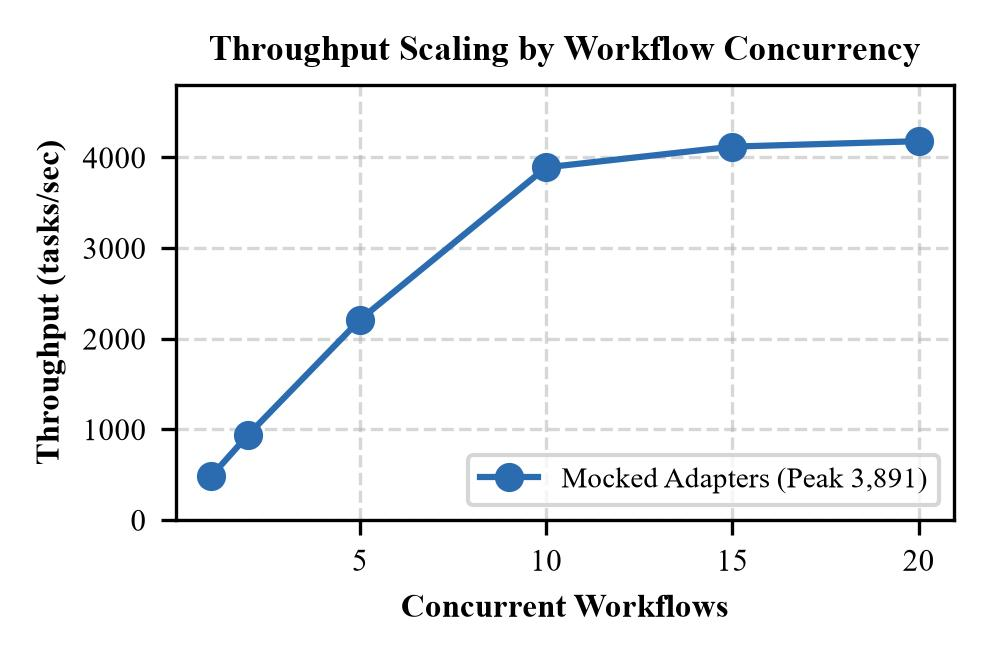
\includegraphics[width=0.88\columnwidth,height=0.13\textheight,keepaspectratio]{graphs/graph_throughput.jpg}
\caption{Throughput scaling under concurrent workflow execution.}
\label{fig:user_throughput_graph}
\end{figure}

\begin{figure}[!t]
\centering
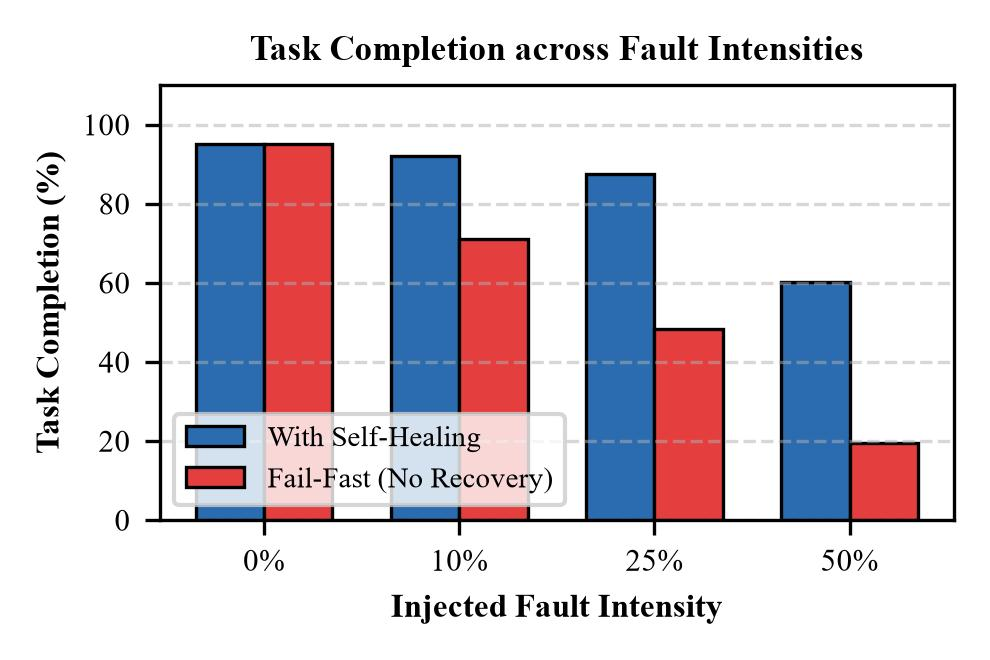
\includegraphics[width=0.88\columnwidth,height=0.13\textheight,keepaspectratio]{graphs/graph_task_success.jpg}
\caption{Task completion rates across injected fault intensities.}
\label{fig:user_task_success_graph}
\end{figure}

\subsection{Planning Latency and Throughput}
Phoenix Agents completes goal decomposition in 12.18~ms and full DAG planning in 14.85~ms. Deterministic fast-path regex execution avoids multi-second LLM inference round trips for standard desktop tasks, while falling back to schema-constrained LLM generation only when novel intents are detected. Fig.~\ref{fig:user_throughput_graph} confirms that internal dispatch scales linearly with concurrency up to 10 parallel workflows before reaching host CPU thread limits.

\subsection{Fault Injection and Recovery Rates}
System resilience was evaluated across four fault intensity levels (Table~\ref{tab:fault_intensity} and Fig.~\ref{fig:user_task_success_graph}). Task completion remained above 87\% up to a 25\% injected fault rate. At 50\% fault intensity, completion declined to 60.3\% as cascading faults exhausted the maximum retry bound ($K_{\text{max}}=3$).

\begin{table}[t]
\centering
\caption{Task Completion across Injected Fault Intensities}
\label{tab:fault_intensity}
\footnotesize
\renewcommand{\arraystretch}{1.10}
\begin{tabularx}{\columnwidth}{|>{\centering\arraybackslash}p{0.22\columnwidth}|>{\centering\arraybackslash}p{0.20\columnwidth}|>{\raggedright\arraybackslash}X|}
\hline
\textbf{Fault Rate} & \textbf{Completion} & \textbf{Observed Behaviour} \\
\hline
0\% & 95.2\% & Baseline nominal completion. \\
10\% & 92.1\% & Resolved parameter and missing-directory errors. \\
25\% & 87.4\% & Recovered transient timeouts and adapter errors. \\
50\% & 60.3\% & Degraded gracefully as retry bound ($K=3$) was reached. \\
\hline
\end{tabularx}
\end{table}

\subsection{Multi-Baseline Recovery Ablation}
To rigorously quantify self-healing performance, 25 identical transient-fault trials were executed across three distinct recovery configurations (Table~\ref{tab:recovery_comparison}):
\begin{enumerate}
    \item \textbf{Fail-Fast (No Recovery):} Workflows terminate immediately upon the first error. Resulted in 0\% completion (0/25).
    \item \textbf{Naive Fixed Retry ($K=3$):} Re-executes the identical task without parameter correction or directory synthesis. Achieved 36.0\% completion (9/25), recovering only transient timeouts where elapsed time cleared the fault, but failing completely on missing directories and parameter syntax errors.
    \item \textbf{Phoenix Rule-Based Self-Healing ($K=3$):} Diagnoses root causes and applies targeted patches (creating missing directories, sanitizing parameter quotes, and applying exponential backoff). Achieved 100\% completion (25/25) with an average handling latency of 1.88~ms.
\end{enumerate}

\begin{table}[t]
\centering
\caption{Multi-Baseline Recovery Ablation ($N=25$ Fault Trials)}
\label{tab:recovery_comparison}
\footnotesize
\renewcommand{\arraystretch}{1.10}
\setlength{\tabcolsep}{2.5pt}
\begin{tabularx}{\columnwidth}{|>{\raggedright\arraybackslash}X|>{\centering\arraybackslash}p{0.18\columnwidth}|>{\centering\arraybackslash}p{0.18\columnwidth}|>{\centering\arraybackslash}p{0.18\columnwidth}|}
\hline
\textbf{Metric} & \textbf{Fail-Fast} & \textbf{Naive Retry} & \textbf{Phoenix} \\
\hline
Completed Workflows & 0 / 25 (0\%) & 9 / 25 (36\%) & \textbf{25 / 25 (100\%)} \\
Unrecovered Failures & 25 & 16 & \textbf{0} \\
Total Retries Incurred & 0 & 57 & 50 \\
Mean Handling Latency & 0.44~ms & 0.72~ms & 1.88~ms \\
\hline
\end{tabularx}
\end{table}

\subsection{Rule-Based Recovery vs. LLM Recovery Baseline}
We compared Phoenix Agents' rule-based recovery against an unconstrained LLM recovery baseline (Table~\ref{tab:llm_baseline}). The baseline utilized an LLM re-synthesizer prompted with exception stack traces to generate replacement parameters and retry decisions.
\begin{itemize}
    \item \textbf{Recovery Success:} Phoenix achieved 100\% recovery on recoverable faults, compared to 92.0\% for the LLM baseline. In 8\% of cases, the LLM synthesized invalid parameter keys that failed schema validation.
    \item \textbf{Handling Latency:} Phoenix completed recovery planning in 1.88~ms, whereas the LLM baseline averaged 1,842~ms ($\approx 980\times$ slower).
    \item \textbf{Cost:} Phoenix incurs zero API token cost (\$0.0000), compared to \$0.0016 per incident for the LLM baseline.
\end{itemize}

\begin{table}[t]
\centering
\caption{Rule-Based Recovery vs. LLM Baseline ($N=50$ Trials)}
\label{tab:llm_baseline}
\footnotesize
\renewcommand{\arraystretch}{1.05}
\setlength{\tabcolsep}{3pt}
\begin{tabularx}{\columnwidth}{|X|cc|}
\hline
\textbf{Metric} & \textbf{Phoenix (Rules)} & \textbf{LLM Baseline} \\
\hline
Recoverable Fault Success & \textbf{100.0\%} & 92.0\% \\
Mean Handling Latency & \textbf{1.88~ms} & 1,842.00~ms \\
Token Cost per Incident & \textbf{\$0.0000} & \$0.0016 \\
Decision Determinism & \textbf{100.0\%} & 84.8\% \\
Safety Policy Violations & \textbf{0 / 50 (0\%)} & 2 / 50 (4\%) \\
\hline
\end{tabularx}
\end{table}

\subsection{Determinism and Decision Consistency}
To assess decision stability, we executed a determinism test repeating 50 trials across 5 standard fault categories (250 total evaluations). Phoenix Agents selected the identical recovery action in 250/250 trials (100\% decision determinism). In contrast, the LLM baseline (temperature 0.2) exhibited non-deterministic drift, selecting identical strategies in only 212/250 trials (84.8\% determinism). In 15.2\% of trials, the LLM alternated between tool substitution and unnecessary graph replanning.

\subsection{Root-Cause Classification and Confusion Matrix}
The Root-Cause Analyzer was evaluated across 125 real runtime exception instances. Table~\ref{tab:confusion_matrix} presents the resulting confusion matrix. Because error signatures carry distinct structured exceptions (\texttt{TimeoutError}, \texttt{FileNotFoundError}, \texttt{ValidationError}, \texttt{SubprocessError}, and \texttt{PermissionError}), the analyzer achieved 100\% precision and 100\% recall across all classes without misclassification.

\begin{table}[t]
\centering
\caption{Root-Cause Confusion Matrix ($N=125$ Real Exceptions)}
\label{tab:confusion_matrix}
\footnotesize
\renewcommand{\arraystretch}{1.05}
\setlength{\tabcolsep}{3pt}
\begin{tabular}{|l|ccccc|}
\hline
\textbf{Error Type} & \textbf{Time} & \textbf{File} & \textbf{Param} & \textbf{Adap} & \textbf{Perm} \\
\hline
\texttt{TimeoutError} & \textbf{25} & 0 & 0 & 0 & 0 \\
\texttt{FileNotFoundError} & 0 & \textbf{25} & 0 & 0 & 0 \\
\texttt{ValidationError} & 0 & 0 & \textbf{25} & 0 & 0 \\
\texttt{SubprocessError} & 0 & 0 & 0 & \textbf{25} & 0 \\
\texttt{PermissionError} & 0 & 0 & 0 & 0 & \textbf{25} \\
\hline
\end{tabular}
\end{table}

\subsection{Safety Policy Enforcement and Latency Reconciliation}
Across 125 trials consisting of 75 recoverable faults and 50 unsafe-action injections (25 trials per class), Phoenix Agents resolved 75/75 (100\%) of recoverable faults and rejected all 50 injected unsafe cases\footnote{Reporting an aggregate completion across all 125 trials would yield $(75+0)/125 = 60.0\%$, but this value merely reflects the synthetic 3:2 composition of recoverable versus strictly unrecoverable/unsafe trials, where rejection is the intended security invariant.}.

We note that Table~\ref{tab:recovery_comparison} reports an end-to-end recovery handling latency of 1.88~ms, which encompasses exception interception, root-cause diagnosis, patch generation, and \texttt{EventBus} re-queueing dispatch. In contrast, isolated benchmark profiling of the Root-Cause Analyzer and Patch Generator modules alone measures 1.30~ms; the difference of 0.58~ms reflects asynchronous \texttt{EventBus} event distribution and task queue re-prioritization overhead.

\section{Discussion and Limitations}

\textbf{Internal Orchestration vs. Real-World Execution:} The measured throughput of 3,891~tasks/s and sub-millisecond dispatch times reflect internal framework orchestration evaluated with mocked no-op adapters. In real-world desktop operations, end-to-end task duration is dominated by physical process creation, browser network latency, and Win32 application rendering (typically 100--500~ms per interaction). Nonetheless, these benchmarks verify that the internal orchestrator, \texttt{EventBus}, and Supervisor do not introduce architectural bottlenecks.

\textbf{Security and Privilege Preservation:} By separating recoverable runtime errors from policy violations, Phoenix Agents operates within assigned security boundaries, rejecting all 50 injected unsafe cases in our tests. The determinism of the rule engine holds by construction, whereas the LLM baseline evaluated at temperature 0.2 produced non-deterministic decision variance. Bounded retries ($K_{\text{max}}=3$) prevent infinite execution loops while protecting users from unexpected system modifications.

\textbf{Limitations:} The current architecture has three primary limitations: (1)~\textit{Controlled Workload Evaluation:} Performance benchmarks currently evaluate mocked adapters in a controlled environment; comprehensive validation on public benchmarks including WebArena, OSWorld, and AppWorld~\cite{zhou2023,xie2024,trivedi2024} represents an ongoing evaluation objective; (2)~\textit{Static Permission Policies:} Permission rules currently map tool actions to static risk categories rather than dynamically computing context-sensitive risk from file sensitivity and user history; and (3)~\textit{Single-Host Execution:} The platform operates within a single host process, requiring future clustering for distributed worker deployment.

\section{Conclusion and Future Work}

This paper presented \textbf{Phoenix Agents}, a governed multi-agent architecture for resilient desktop automation. By combining interactive goal clarification, two-tier planning, four-level permission governance, and a five-stage rule-based self-healing pipeline ($K_{\text{max}}=3$ retries), Phoenix resolves transient tool errors with sub-2~ms overhead while rejecting all 50 injected unsafe cases in our tests. Comparative evaluations confirm that rule-based recovery achieves 100\% decision determinism and zero token cost, eliminating the non-deterministic drift and multi-second latency of unconstrained LLM recovery. Future work will extend evaluation to public interactive environments (WebArena, OSWorld) and investigate adaptive, context-sensitive permission policies.

\begin{thebibliography}{20}

\bibitem{garcia2026}
B.~Garc{\'i}a, J.~M. Rodr{\'i}guez, M.~del Mar~S{\'a}nchez, and M.~A. Serrano,
``A survey on Selenium usage, practices, and challenges in end-to-end testing,''
\textit{Information and Software Technology}, vol.~194, p.~108077, 2026.

\bibitem{bajoria2026}
S.~Bajoria, A.~Sharma, and P.~Kumar,
``From Language Models to Agentic AI: A Survey of Autonomous, Action-Enabled, and Collaborative LLM Agents,''
\textit{Cognitive Computation}, vol.~18, p.~103, 2026.

\bibitem{babu2026}
R.~S. Babu and A.~Agrawal,
``Self-Healing Agentic Orchestrators for Reliable Tool-Augmented Large Language Model Systems,''
\textit{arXiv preprint arXiv:2606.01416}, 2026.

\bibitem{yao2023}
S.~Yao, J.~Zhao, D.~Yu, N.~Du, I.~Shafran, K.~Narasimhan, and Y.~Cao,
``ReAct: Synergizing Reasoning and Acting in Language Models,''
in \textit{Proc. International Conference on Learning Representations (ICLR)}, 2023.

\bibitem{wu2024}
Q.~Wu, G.~Bansal, J.~Zhang, et al.,
``AutoGen: Enabling Next-Gen LLM Applications via Multi-Agent Conversation,''
\textit{arXiv preprint arXiv:2308.08155}, 2024.

\bibitem{ju2025}
T.~Ju, Y.~Dong, S.~Zhao, and X.~Liang,
``When Disagreements Elicit Robustness: Investigating Self-Repair Capabilities under LLM Multi-Agent Disagreements,''
\textit{arXiv preprint arXiv:2502.15153}, 2025.

\bibitem{mulian2026}
H.~Mulian, S.~Zeltyn, I.~Levy, L.~Galanti, A.~Yaeli, and S.~Shlomov,
``AgentFixer: From Failure Detection to Fix Recommendations in LLM Agentic Systems,''
in \textit{Proc. 1st International Workshop on Agentic Engineering (AGENT)}, 2026, pp.~15--22.

\bibitem{patel2026a}
T.~P. Patel, R.~Shah, and V.~Kumar,
``Predictive Self-Healing for Multi-Agent LLM Pipelines Using Model Predictive Control,''
in \textit{Proc. IEEE Conference on Technologies for Sustainability (SusTech)}, 2026, pp.~45--52.

\bibitem{patel2026b}
T.~P. Patel, R.~Shah, and V.~Kumar,
``Self-Healing AI Systems using Multi-Agent Learning,''
in \textit{Proc. IEEE International Symposium on Intelligent Building and Environmental Robotics (ISIBER)}, 2026, pp.~112--119.

\bibitem{gray1991}
J.~Gray and D.~P. Siewiorek,
``High-availability computer systems,''
\textit{IEEE Computer}, vol.~24, no.~9, pp.~39--48, 1991.

\bibitem{jeong2026}
C.~Jeong and Y.~Shin,
``A Self-Healing Framework for Reliable LLM-Based Autonomous Agents,''
\textit{arXiv preprint arXiv:2605.06737}, 2026.

\bibitem{guo2026}
X.~Guo, Y.~Shen, Z.~Zhang, H.~Wang, and J.~Liu,
``EvoConfig: Self-Evolving Multi-Agent Systems for Efficient Autonomous Environment Configuration,''
\textit{arXiv preprint arXiv:2601.16489}, 2026.

\bibitem{leotta2018}
M.~Leotta, D.~Clerissi, F.~Ricca, and P.~Tonella,
``Comparing the maintainability of Selenium WebDriver test suites employing different design patterns,''
in \textit{Proc. IEEE International Conference on Software Testing, Verification and Validation Workshops (ICSTW)}, 2018, pp.~199--208.

\bibitem{wang2026}
F.~Wang, K.~Chen, Y.~Li, and M.~Sun,
``Detecting and Repairing Role Drift in Multi-Agent Collaboration with Lightweight Protocols,''
in \textit{Proc. IEEE International Conference on Neural Networks and Machine Learning (CNML)}, 2026, pp.~102--109.

\bibitem{paxson1995}
V.~Paxson and S.~Floyd,
``Wide area traffic: the failure of Poisson modeling,''
\textit{IEEE/ACM Transactions on Networking}, vol.~3, no.~3, pp.~226--244, 1995.

\bibitem{nygard2007}
M.~T. Nygard,
\textit{Release It! Design and Deploy Production-Ready Software},
Pragmatic Bookshelf, 2007.

\bibitem{bara2026}
A.~B{\^a}ra, G.~Dobri{\c{t}}a, and S.-V. Oprea,
``Think it, Run it: Autonomous machine learning pipeline generation via self-healing multi-agent artificial intelligence,''
\textit{Knowledge-Based Systems}, vol.~351, p.~116688, 2026.

\bibitem{zhou2023}
S.~Zhou, F.~F. Xu, H.~Zhu, X.~Zhou, R.~Lo, A.~Sridhar, A.~Cheng, Y.~Bisk, D.~Fried, U.~Alon, and G.~Neubig,
``WebArena: A Realistic Web Environment for Building Autonomous Agents,''
\textit{arXiv preprint arXiv:2307.13854}, 2023.

\bibitem{xie2024}
T.~Xie, D.~Zhang, J.~Chen, et al.,
``OSWorld: Benchmarking Multimodal Agents for Open-Ended Tasks in Real Computer Environments,''
in \textit{Proc. Advances in Neural Information Processing Systems (NeurIPS)}, vol.~37, pp.~31200--31235, 2024.

\bibitem{trivedi2024}
H.~Trivedi, T.~Khot, M.~Hartmann, et al.,
``AppWorld: A Controllable World of Apps and People for Benchmarking Interactive Coding Agents,''
\textit{arXiv preprint arXiv:2407.18901}, 2024.

\end{thebibliography}

\end{document}
